\section{Visione Artificiale}
La visione dell'ambiente circostante è la questione focale nello sviluppo di un veicolo a guida autonoma. Per poter "vedere", una macchina utilizza diversi sensori:
\begin{itemize}
    \item  Camere
    \item Radar
    \item Lidar
\end{itemize}
\begin{figure}[h]
    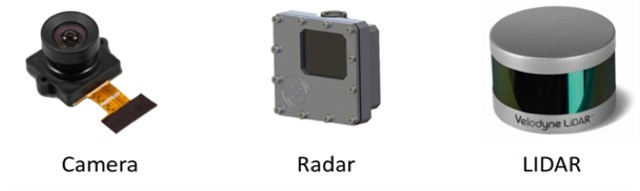
\includegraphics[width = \linewidth]{sensori.jpg}
    \caption{i sensori più utilizzati\cite{lid}}
    \label{fig:lid}
\end{figure}
\subsection{Camere}
Le videocamere utilizzate sono profondamente diverse dalle normali videocamere in vendita. Sono progettate in modo da avere un campo visivo molto ampio, migliore sensibilità anche a bassa luminosità,
bassa risoluzione(migliori performance) e per funzionare ad alte  e basse temperature. Restano però limitate in situazioni di bassa visibilità.     
\subsection{Radar}
Il compito dei radar è principalmente quello di rilevare ostacoli e situazioni di pericolo imminente. In base alle informazioni raccolte l'auto accelera o frena. 
I radar si rilevano utili anche nella fase di parcheggio.
\subsection{Lidar}
I lidar sono dispositivi il cui funzionamento è simile a quello dei radar. La differenza principale sta nel segnale utilizzato: i radar usano onde radio mentre i lidar usano impulsi luminosi.
I lidar sono particolarmente utili per la rilevazione di pedoni e per riconoscere i segnali stradali.
\begin{figure}[h!]
    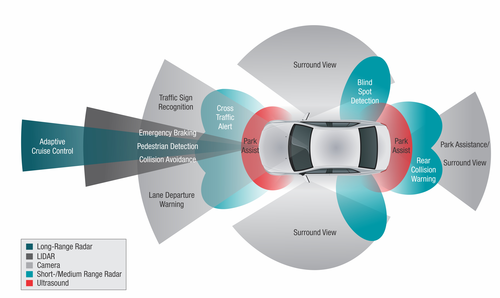
\includegraphics[scale=0.6]{01-autonomous-car-sensors_TI.png}
    \caption{sensori in una macchina autonoma\cite{sensors}}
    \label{fig:sensors}
\end{figure}
\newpage
\subsection{Dai sensori agli attuatori}

Tutti i sensori sono fondamentali perchè ciascuno di esso compensa i punti deboli dell'altro. Una videocamera non funziona bene in condizioni di nebbia intensa, ma un radar sì. Un radar però non riconosce se
un semaforo è verde o rosso, mentre una camera sì. Nella figura \ref{fig:sensors} sono mostrate le funzioni svolte da ciascun sensore.


Le informazioni raccolte dai sensori vengono passate al "livello" sottostante, nel quale il sistema interno sceglie la prossima azione da compiere.
Il modello decisionale più utilizzato è una rete neurale convoluzionale. Il deep learning si è dimostrato estremamente potente in quest'ambito, fornendo
ottimi risultati per l'object recognition. L'azione scelta viene passata agli attuatori(freno, sterzo, acceleratore) che provvedono ad eseguirla.
\begin{figure}[h]
    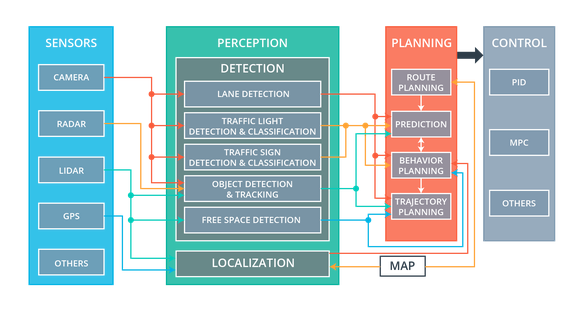
\includegraphics[width=\linewidth]{plan.png}
    \caption{Il processo decisionale\cite{giacaglia}}
    \label{fig:giacaglia}
\end{figure}